% !TeX root = RJwrapper.tex
\title{\pkg{OneStep} : Le~Cam's One-step Estimation Procedure}
\author{by Alexandre Brouste, Christophe Dutang and Darel Noutsa Mieniedou}

\maketitle

\abstract{
The \pkg{OneStep} package proposes principally an eponymic function that numerically computes Le Cam's one-step estimator, which is asymptotically efficient and can be computed faster than the maximum likelihood estimator for large datasets. Monte Carlo simulations are carried out for several examples (discrete and continuous probability distributions) in order to exhibit the performance of Le Cam's one-step estimation procedure in terms of efficiency and computational cost on observation samples of finite size. 
}

\section{Introduction}

In the statistical experiments generated by i.i.d.~observation samples, the sequence of maximum likelihood estimators (MLE) is known to be asymptotically efficient under very general assumptions and consequently presents the fastest convergence rate and the lowest possible asymptotic variance.

Although the sequence of MLE is asymptotically efficient, it is generally not expressed in a closed form and requires time consuming numerical computations. On the other hand, the other generic estimation procedures which can sometimes be computed faster, as the method of moments, do not generally reach the optimal asymptotic variance.

In R, the package \pkg{fitdistrplus} (see \cite{fitdistrplus15}) is commonly used to infer the parameters 
of univariate probability distributions.
For non-censored datasets, \pkg{fitdistrplus} allows four  different  estimation  methods: 
maximum likelihood, moment matching, quantile matching, and maximum goodness-of-fit estimation.
The unified approach is provided by \code{fitdist()} which returns an S3-object having usual generic functions
(\code{plot}, \code{summary}, \code{logLik}, \dots) as well as dedicated \code{fitdist}-functions
(\code{gofstat}, \code{bootdist}, \dots).

Other packages with similar purposes are  \pkg{EstimationTools} and \pkg{DistributionFitR}, 
providing MLE for non-censored data. Many other packages also provide estimation procedure on the 
basis of one function per probability distribution; see, e.g., packages \pkg{univariateML}, \pkg{propagate}.
A final package, which is worth mentioning, is \pkg{fitter}, which fits a set of probability distributions 
on a given dataset sequentially.

However, as soon as the Fisher information matrix is sufficiently regular with respect to the parameter to be estimated, Le Cam's one-step estimation procedures can be achieved (see \cite{LeCam}). They are based on an initial sequence
of guess estimators and a single Newton step or a Fisher scoring step on the loglikelihood function. Namely, they write
\begin{equation}\label{LC1}
 \overline{\vartheta}_n  =   \vartheta^*_n  + {\cal I}(\vartheta^*_n)^{-1}\cdot \frac1n \sum_{j=1}^n \dot{\ell} (\vartheta^*_n,X_j), \quad n \geq 1,
\end{equation}
for the Fisher scoring type procedure, where $(\vartheta^*_n, n \geq 1)$ is the initial sequence of guess estimators, $\ell(\vartheta)$ is the loglikelihood function, the dot is the notation for the gradient with respect to $\vartheta$, and ${\cal I}(\vartheta)=-\Es_\vartheta( \ddot{\ell} (\vartheta) )$ is the Fisher information matrix and
\begin{equation}\label{LC2}
 \overline{\vartheta}_n  =   \vartheta^*_n  + \widehat{{\cal I}}_n(\vartheta^*_n)^{-1}\cdot \frac1n \sum_{j=1}^n \dot{\ell} (\vartheta^*_n,X_j), \quad n \geq 1,
\end{equation}
for the Newton type procedure, where $\widehat{{\cal I}}_n(\vartheta)= -\frac{1}{n}\sum_{j=1}^n \ddot{\ell} (\vartheta,X_j)$ is the opposite of the Hessian for the loglikelihood function.


The sequence of Le Cam's one-step estimators presents certain advantages over the sequence of MLE and over the initial sequence of estimators (method of moments, quantile matching method, etc.) in terms of computational cost and asymptotic variance. 
It is much less computationally expensive than the MLE, while it has the same rate and the same asymptotic variance. 
Since there is no full numerical optimization (but only one computation of the Newton step or the Fisher scoring step), the procedure 
is faster and appropriate for very large datasets.
On the other hand, it is asymptotically  optimal in terms of asymptotic variance, which is generally not 
the case for the initial sequence of guess estimators. 


For several probability distributions (Gaussian, Exponential, Lognormal, Poisson, Geometric), a fast computable sequence of estimators is already asymptotically efficient, and no correction is needed. When the Fisher information is given in a closed form (Gamma, Beta, $\chi^2$, Weibull, Pareto II, Cauchy), Le~Cam's one-step estimation procedure~\eqref{LC1} is executed.  In all the other cases, the estimation procedure~\eqref{LC2} is used either with the score function and the Hessian in a closed form (Negative Binomial) or with the numerical approximation of the score function and the Hessian with the package \pkg{numDeriv} (see \cite{numDeriv19}).

Le Cam's one-step estimation procedures are implemented in the package \pkg{OneStep}, and the eponymic function \pkg{onestep} is described in this paper and used on different examples. Monte Carlo simulations are performed for several examples in order to exhibit the performance of Le Cam's one-step procedure on samples of finite size. They exhibit their asymptotic efficiency simultaneously with their better computational cost for several probability distributions.

\section{The function \code{onestep}}

Let $(X_1,X_2, \ldots, X_n)$ be a sample of i.i.d. random variables. The probability density function of $X_1$ is denoted $f$ and depends on an unknown parameter $\vartheta \in \Theta \subset \mb{R}^p$ which is to be estimated.

Le~Cam's one-step estimation procedure is based on an initial sequence of guess estimators and a Fisher scoring step or a single Newton step on the loglikelihood function. For the novice user, the function \pkg{onestep} automatically chooses the best procedure to be used. There is, consecutively, a single command for the user, which is 

\code{onestep(data, distr)}

The function \pkg{onestep} presents several procedures internally depending on whether the initial sequence of guess estimators is in a closed-form or not and whether the score and the Fisher information matrix can be elicited in a closed-form.

Here is the list of the procedures taken into account in the \pkg{onestep} function:
\begin{enumerate}
\item Distributions for which the MLE is already explicit: \code{norm}, \code{exp}, \code{lnorm}, \code{invgauss} for continuous probability distributions, and \code{pois}, \code{geom} for discrete probability distributions. For this class, the explicit MLE is returned.
\item Distributions for which the initial sequence of guess estimators, the score and the Fisher information matrix have been elicited in a closed-form: \code{gamma}, \code{beta}, \code{chisq} with an initial sequence of moment estimators, \code{cauchy} with an initial sequence of quantile matching estimators, and \code{weibull} with an initial sequence of graphical plot estimators. For this class, Le Cam's one-step procedure \eqref{LC1} is applied.
\item Distributions for which the initial sequence of guess estimators, the score, and the Hessian have been elicited in a closed-form: \code{nbinom}. For this class, Le Cam's one-step procedure \eqref{LC2} is applied.
\item Distributions for which the initial sequence is numerically computed on a subsample, but the score and the Fisher information matrix have closed-form: \code{pareto}. For this class,  Le Cam's one-step procedure \eqref{LC1} is executed.
\item For all other distributions, if the density function is well defined, the numerical computation of the Newton step in  Le Cam's one-step procedure \eqref{LC2} is proposed with an initial sequence of guess estimators, which is the sequence of maximum likelihood estimators computed on a subsample.
\end{enumerate}


As is described, all explicit distributions of the \code{mmedist} function from
\pkg{fitdistrplus} have been corrected in the \pkg{onestep} function, except
\code{unif} and \code{logis}. The example \code{unif} is a famous example of the singular behavior of the MLE. The correction of \code{logis} is of very small gain from the method of moments estimator to the MLE. For these two distributions, the method of moments is returned.

However, the package also offers several new explicit computations as \code{cauchy}, \code{chisq} and \code{weibull} and applies to distributions coming from the \pkg{actuar} package (see \cite{actuar08}) 
such as \code{invgauss} and \code{pareto}.

The function \code{onestep} allows the user to propose its own initial guess estimation in the one-step procedure by specifying the parameter \code{init} in the command

\code{onestep(data, distr, init)}

The user can consequently use different initial guess estimators for the aforementioned classical distributions (moment estimators, estimators based on the characteristic function, quantile matching estimators, Bayesian estimators, mode-type estimators, graphical methods, {\it etc.}). Several examples can be found in the documentation of the \code{onestep} function.

Monte Carlo simulations are done for several examples (discrete and continuous probability distributions) in order to exhibit the performance of Le Cam's one-step estimation procedure in terms of efficiency and computational cost on observation samples of finite size. 

For the assessment of the efficiency, the proximity of the renormalized statistical errors $(Y_1,Y_2,\ldots, Y_M)$ to the centered Gaussian asymptotic distribution (for a coordinate in the multivariate setting) is evaluated with the Cramer-Von Mises statistic 
$$ T= M \omega^2_M = M \int_\mathbb{R} \left(F_M(y)-F_*(y) \right)^2 dF_*(y) = \frac{1}{12M} + \sum_{i=1}^M  \left(F_*(Y_{(i)})- \frac{2i-1}{2M}\right)^2,$$
where the order statistics are denoted $Y_{(1)} \leq Y_{(2)} \leq \dots \leq  Y_{(M)}$, $F_*(\cdot)$ is the theoretical Gaussian asymptotic cumulative distribution function and 
$$F_M(y)=\frac{1}{M}\sum_{i=1}^M \mathbbm{1}_{\{ Y_i \leq y \}}$$
is the empirical cumulative distribution function. The asymptotic distribution of $T$ is tabulated, for instance, in the \code{goftest} package. Note that a value of the statistic below 0.7434 corresponds to accept the null (and the equivalence to theoretical Gaussian asymptotic distribution) with an error of type I equal to 1\%. 

Timing performance (given in seconds) is done with the \code{proc.time}  function (\code{"elapsed"} time) on a laptop with an Intel Core i7 2.7 GHz processor with 8GB RAM. The \code{onestep} function is compared to the MLE computed with \code{mledist} of the \pkg{fitdistrplus} package and to the sequence of initial guess estimators (for instance, the moment estimator is computed with \code{mmedist} for the \code{gamma}, \code{beta}, and \code{nbinom} distributions).

The functions \code{benchonestep} and  \code{benchonestep.replicate} were used  to compare the performance of estimators (see documentation of the \pkg{OneStep} package).

\subsection{Closed-form sequence of initial guess estimators}\label{sec:closed}

For the majority of the "closed formula" cases, the initial sequence of guess estimators of the unknown parameter $\vartheta$ is the sequence of moment estimators. 

Let $(X_1,X_2, \ldots, X_n)$ be a sample of i.i.d. random variables. Let us denote the theoretical moments $m_k(\vartheta)=\Es_\vartheta (X_1^k)$ and the empirical moments $\tilde{m}_k=\frac{1}{n} \sum_{j=1}^n X_j^k$. The sequence of moment estimators (ME) is generally defined as the solution of the system of equations 
$$m_k(\vartheta_n^*) =\tilde{m}_k , \quad k=1,\ldots,p.$$
Indeed, under very mild conditions, the sequence of moment estimators $(\vartheta_n^*, n\geq 1)$ is asymptotically normal, and therefore,  $\sqrt{n}$-consistent (see \cite{IK}). Namely,
\begin{equation}\label{eq:normME} \sqrt{n} \left( \vartheta_n^* - \vartheta \right) \longrightarrow {\cal N}\left(0, J^{-1}(\vartheta) A(\vartheta) J^{-T}(\vartheta)\right)
\end{equation}
in law as $n\rightarrow \infty$, where 
$$J(\vartheta)= \left( \frac{\partial}{\partial \vartheta_j} m_i(\vartheta) \right)_{1\leq i\leq p, 1 \leq j \leq p}$$ 
and 
$$A(\vartheta)=\Es_\vartheta \left( (X_1^i - m_i(\vartheta))(X_1^j - m_j(\vartheta)) \right)_{1\leq i\leq p, 1 \leq j \leq p}.$$
Here, the notation $M^T$ means the transpose matrix of $M$. Several examples (Gamma, Beta, and Negative Binomial) are given later on in this section. 

However, other $\sqrt{n}$-consistent sequences of initial guess estimators can be used. For instance, an initial sequence of quantile matching estimators is employed for the Cauchy distribution.

It had been shown in \cite{LeCam} that for a $\sqrt{n}$--consistent initial sequence of guess estimators and an uniformly continuous Fisher information matrix, the sequence of Le Cam's one-step estimators
defined in \eqref{LC1} or \eqref{LC2} is consistent, asymptotically normal and efficient (in the Fisher sense) with
$$ \sqrt{n}\left( \widehat{\vartheta}_n-\vartheta \right) \rightarrow {\cal N}\left(0,{\cal I}(\vartheta)^{-1}\right).$$
In other words, for an initial sequence which is asymptotically rate but not variance efficient, the new sequence is asymptotically rate and variance efficient. 


\paragraph{Gamma}

The first example is the joint estimation of the shape parameter $\alpha$  and scale parameter $\beta$ in the statistical experiment generated by a sample $(X_1,X_2,\ldots,X_n)$ of i.i.d. Gamma random variables whose probability density function is given by
$$ f(x)= \frac{\beta^\alpha}{\Gamma(\alpha)}x^{\alpha-1} \exp( - \beta x ), \quad x >0.$$

Let us denote $\vartheta=(\alpha,\beta)$. In this statistical experiment, the sequence of maximum likelihood estimators $(\widehat{\vartheta}_n, n \geq 1)$ of $\vartheta$ is not in a closed-form.  The sequence of MLE satisfies 
$$ \sqrt{n}\left( \widehat{\vartheta}_n-\vartheta \right) \rightarrow {\cal N}\left(0,{\cal I}(\vartheta)^{-1}\right),$$
where 
$$ {\cal I}(\vartheta)=\begin{pmatrix} \psi^{(2)}(\alpha) & -\frac{1}{\beta} \\ - \frac{1}{\beta} &  \frac{\alpha}{\beta}\end{pmatrix}.$$
Here, $\psi^{(n)}$ is the polygamma functions (see  \cite[section 6.4.1, page 260]{AS72}) defined by $\psi^{(n)}(\alpha)=\frac{\partial^n}{\partial \alpha^n} \log \Gamma(\alpha)$. Consider that 
$$ m_k(\vartheta) = \frac{\alpha(\alpha+1) \ldots (\alpha+k-1)}{\beta^n}.$$
Consecultively, the sequence of moment estimators  $(\vartheta^*_n=(\alpha^*_n,\beta^*_n), n \geq1)$  given by
$$\alpha^*_n=\frac{\tilde{m}_1^2}{\tilde{m}_2-\tilde{m}_1^2} \quad \mbox{and} \quad \beta^*_n=\frac{\tilde{m}_1}{\tilde{m}_2-\tilde{m}_1^2}$$
is asymptotically normal (see \eqref{eq:normME})
%$$ \sqrt{n} \left( \vartheta^*_n-\vartheta \right) \rightarrow {\cal N}\left(0,J^{-1} A(\vartheta) J^{-*}\right) $$
with  
$$ \quad J=\begin{pmatrix}  \frac{1}{\beta} &  -\frac{\alpha}{\beta^2}  \\ \frac{1+2\alpha}{\beta^2}  & -\frac{2 \alpha(\alpha +1)}{\beta^3}  \end{pmatrix} \quad  \mbox{and}  \quad A(\vartheta)=\begin{pmatrix} \frac{\alpha}{\beta^2} & \frac{2 \alpha(\alpha +1)}{\beta^3} \\ \frac{2 \alpha(\alpha +1)}{\beta^3} & \frac{\alpha (4\alpha+6) (\alpha+1)}{\beta^4}\end{pmatrix},$$
and consequently does not reach asymptotical efficiency.

We can see in Figure~\ref{fig:gamma} (and in Table \ref{tab:gamma:time:cvm} with the Cramer-Von Mises statistics) that the sequence of Le~Cam's one-step estimators (LCE) reaches efficiency and naturally overperforms the initial sequence of ME in terms of asymptotic variance. Moreover, this sequence is faster to be computed on $M=10000$ Monte Carlo simulations than the sequence of MLE, as shown in Table \ref{tab:gamma:time:cvm}, displaying total computation times over $M$. 

\begin{figure}[ht]
\centering
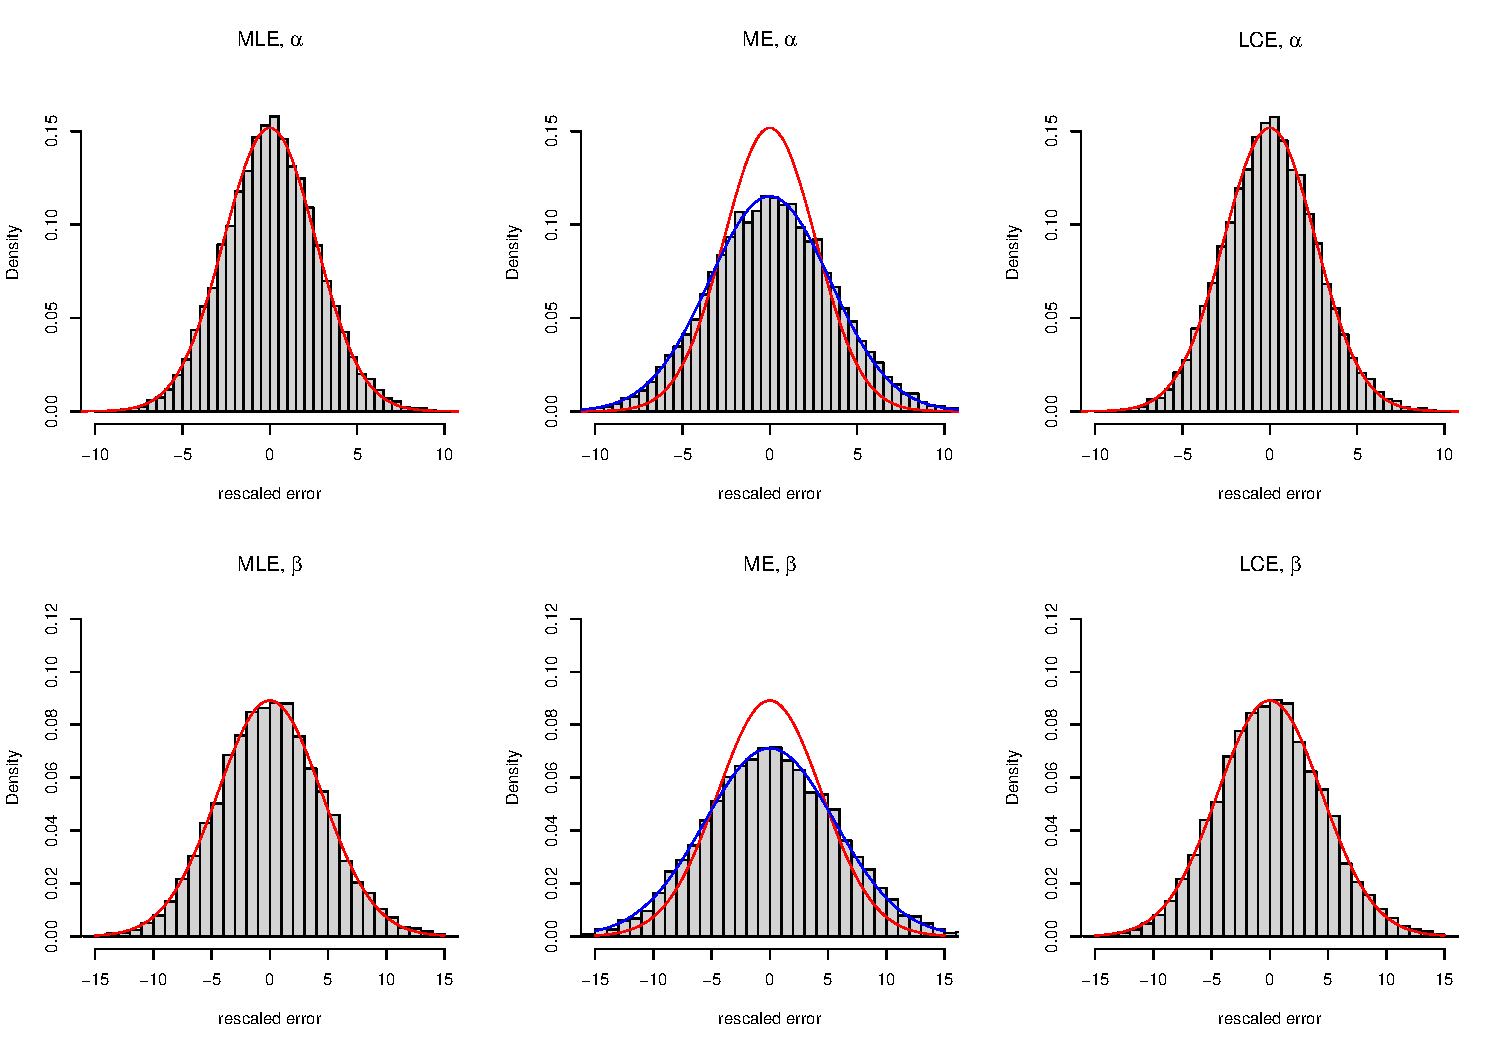
\includegraphics[width=\textwidth]{fig-Gamma.pdf}
\caption{Histograms for the $M=10000$ Monte Carlo simulations of the rescaled statistical error of the MLE, ME, and LCE for the Gamma distribution with $(\alpha,\beta)=(2,3)$ and $n=10000$. Superimposed red and blue lines are the theoretical centered Gaussian asymptotic distributions of the MLE and the ME, respectively.}\label{fig:gamma}
\end{figure}

%\begin{table}[ht]
\input{tab-Gamma.tex}
%\caption{Computation times for MLE, LCE and ME for the Gamma distribution}\label{tab:CPUgamma}
%\end{table}

As it was mentioned in the introduction, the major
advantage of the sequence of one-step estimators is that it is computed faster than the maximum likelihood estimator for large datasets. We illustrate this fact in Table \ref{tab:gamma:time:varying:size}, where the average computation times (over 10 Monte Carlo simulations) are done for different sample sizes $n=10^r$, $r=3,\ldots,9$ for both MLE and LCE. LCE is between 20 times and 55 times faster than MLE, especially for large sample sizes when there is memory overload.

% latex table generated in R 4.0.3 by xtable 1.8-4 package
% Fri Jan 15 21:55:56 2021
\begin{table}[ht]
\centering
\begin{tabular}{rrrrrrrr}
  \hline
 & 10\verb|^|3 & 10\verb|^|4 & 10\verb|^|5 & 10\verb|^|6 & 10\verb|^|7 & 10\verb|^|8 & 10\verb|^|9 \\ 
  \hline
MLE & 0.0121 & 0.1193 & 1.0056 & 10.4735 & 99.4203 & 2339.0437 & 31600.8313 \\ 
  LCE & 0.0007 & 0.0053 & 0.0252 & 0.2361 & 2.3152 & 40.0440 & 540.7393 \\ 
   \hline
\end{tabular}
\caption{Average computation time (s)} 
\label{tab:gamma:time:varying:size}
\end{table}


\paragraph{Beta}

The second example is the joint estimation of the first shape parameter $\alpha$ and the second shape parameter $\beta$ in the statistical experiment generated by a sample $(X_1,X_2,\ldots,X_n)$ of i.i.d. Beta random variables whose probability density function is given by
$$ f(x)= \frac{\Gamma(\alpha+\beta)}{\Gamma(\alpha)\Gamma(\beta)}x^{\alpha-1} (1-x)^{\beta-1}, \quad x \in [0,1].$$

Let us denote $\vartheta=(\alpha,\beta)$. In this statistical experiment, the sequence of maximum likelihood estimators $(\widehat{\vartheta}_n, n \geq 1)$ of $\vartheta$ is not in a closed-form.  The sequence of MLE satisfies 
$$ \sqrt{n}\left( \widehat{\vartheta}_n-\vartheta \right) \rightarrow {\cal N}\left(0,{\cal I}(\vartheta)^{-1}\right),$$
where 
$$ {\cal I}(\vartheta)=\begin{pmatrix} \psi^{(2)}(\alpha) - \psi^{(2)}(\alpha+\beta)& -\psi^{(2)}(\alpha+\beta) \\ - \psi^{(2)}(\alpha+\beta) &  \psi^{(2)}(\beta) - \psi^{(2)}(\alpha+\beta)\end{pmatrix}.$$

It is worth mentioning that for the Beta distribution 
$$ m_k(\vartheta) = \frac{\Gamma(\alpha+k)\Gamma(\alpha+\beta)}{\Gamma(\alpha)\Gamma(\alpha+\beta+k)}$$
that allows one to build closed-form moment estimators. Namely, denoting
$\tilde{w}_n= \frac{\tilde{m}_1(1-\tilde{m}_1)}{\tilde{m}_2-\tilde{m}_1^2} -1$, we obtain
$$\alpha^*_n= \tilde{m}_1 \tilde{w}_n \quad \mbox{and} \quad \beta^*_n= (1-\tilde{m}_1 )  \tilde{w}_n.$$ 
Asymptotic variance in \eqref{eq:normME} of the sequence of moment estimators $(\vartheta^*_n=(\alpha^*_n,\beta^*_n), n \geq1)$ can also be computed with
$$ \quad J=\begin{pmatrix}  \frac{\beta}{(\alpha+\beta)^2} &   -\frac{\alpha}{(\alpha+\beta)^2}  \\  \frac{2\alpha^2\beta+2\alpha \beta^2 + 2\alpha \beta +\beta^2 +\beta}{(\alpha+\beta)^2(\alpha+\beta+1)^2}  &  - \frac{ \alpha(\alpha +1)(2\alpha+2\beta+1)}{(\alpha+\beta)^2(\alpha+\beta+1)^2}  \end{pmatrix}$$
and
$$ A(\vartheta)=\begin{pmatrix} \frac{\alpha\beta}{(\alpha+\beta)^2(\alpha+\beta+1)} & \frac{2 \alpha \beta(\alpha +1)}{(\alpha+\beta)^2(\alpha+\beta+1)(\alpha+\beta+2)} \\ \frac{2 \alpha \beta(\alpha +1)}{(\alpha+\beta)^2(\alpha+\beta+1)(\alpha+\beta+2)} & \frac{\alpha(\alpha+1)(2\alpha^3+6\alpha^2\beta+4\alpha\beta^2+14\alpha\beta+4 \alpha^2+4\alpha+6\beta^2+6\beta)}{(\alpha+\beta)^2(\alpha+\beta+1)(\alpha+\beta+2)(\alpha+\beta+3)}\end{pmatrix},$$
and consequently the sequence does not reach asymptotical efficiency.

Here again, the sequence of Le~Cam's one-step estimators naturally overperforms the initial sequence of ME in terms of asymptotic variance (see Figure~\ref{fig:beta} and the next Table for CvM statistics). 

\begin{figure}[ht]
\centering
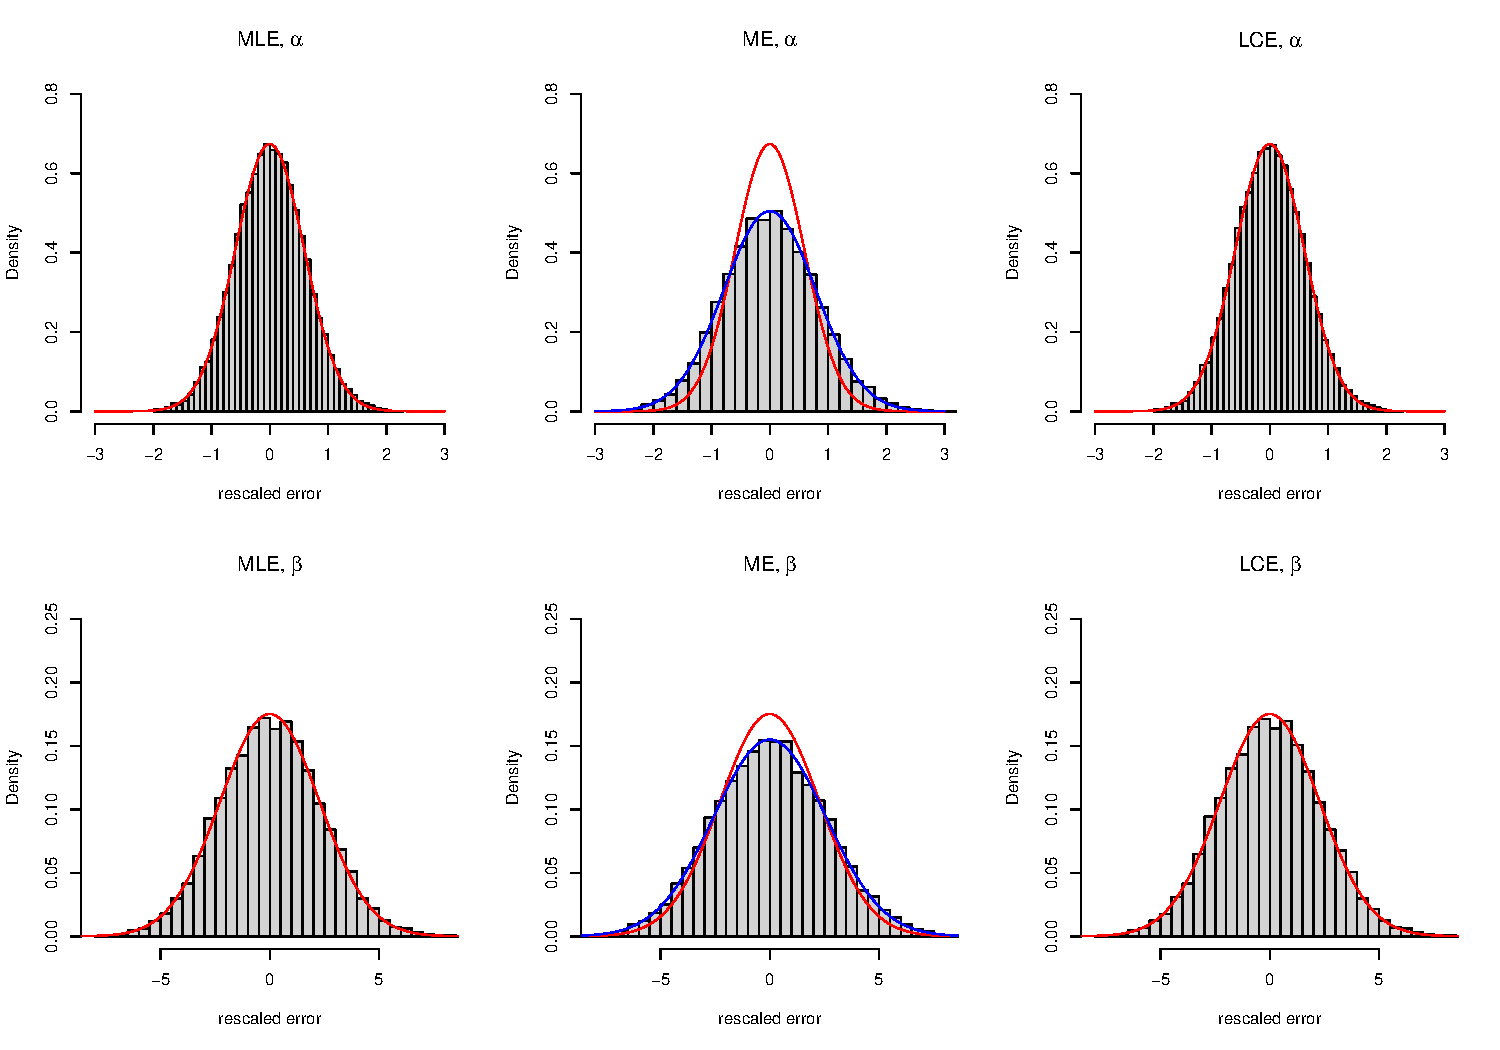
\includegraphics[width=\textwidth]{fig-Beta.pdf}
\caption{Histograms for the $M=10000$ Monte Carlo simulations of the rescaled statistical error of the MLE, ME, and LCE for the Beta distribution with $(\alpha,\beta)=(0.5,1.5)$ and $n=10000$. Superimposed red and blue lines are the theoretical centered Gaussian asymptotic distributions of the MLE and the ME, respectively.}\label{fig:beta}
\end{figure}

It is computed faster than the sequence of MLE, as shown in Table \ref{tab:beta:time:cvm}.


% latex table generated in R 4.0.3 by xtable 1.8-4 package
% Wed Jan  6 17:09:18 2021
\begin{table}[ht]
\centering
\begin{tabular}{rrrr}
  \hline
 & MLE & ME & LCE \\ 
  \hline
Computation time (s) & 2324.99 & 43.26 & 52.02 \\ 
  CvM statistic alpha & 0.22 & 0.06 & 0.05 \\ 
  CvM statistic beta & 0.34 & 0.11 & 0.20 \\ 
   \hline
\end{tabular}
\caption{Computation time and CvM statistics} 
\label{tab:beta:time:cvm}
\end{table}



\paragraph{Cauchy}The third example is the joint estimation of the location parameter $m\in\mb{R}$ and the scale parameter $d>0$ in the statistical experiment generated by a sample $(X_1,X_2,\ldots,X_n)$ of i.i.d. Cauchy random variables whose probability density function is given by
\begin{equation}\label{cauchy}
 f(x) = \frac{d}{\pi \left(d^2+\left(x-m\right)^2\right)}, \quad x \in \mb{R}.
\end{equation}
Let us denote $\vartheta=(m,d)$. In this statistical experiment, the sequence of maximum likelihood estimators $(\widehat{\vartheta}_n, n \geq 1)$ of $\vartheta$ is not in a closed-form.  The sequence of MLE satisfies 
$$ \sqrt{n}\left( \widehat{\vartheta}_n-\vartheta \right) \rightarrow {\cal N}\left(0,{\cal I}(\vartheta)^{-1}\right),$$
where 
$$ {\cal I}(\vartheta)=\begin{pmatrix}\frac{1}{2d^2} & 0 \\ 0&  \frac{1}{2d^2}\end{pmatrix}.$$

It is worth mentioning that the Cauchy distribution has no first moment, and consecutively its unknown parameter $\vartheta$ cannot be estimated via the classical method of moments. But a quantile matching method allows one to define
\begin{equation}
m^*_{n} = Q_n \left(\frac{1}{2}\right) \quad  \mbox{and} \quad d^*_n= \frac12 \left( Q_n \left(\frac{3}{4}\right) -Q_n \left(\frac{1}{4}\right) \right),
\end{equation}
where the sample quantile is usually computed for $p\in(0,1)$ as
$$
Q_n(p) = X_{(\lfloor np\rfloor)},
$$
with the order statistics denoted $X_{(1)} \leq X_{(2)} \leq \dots \leq  X_{(n)}$. 
%There exists advanced formula for computing the sample quantile, generally as a convex combination of X(⌊np⌋) and X(⌊np⌋+1), see e.g. Hyndman & Fan (1996).
This sequence of estimators $(\vartheta^*_n=(m^*_n,d^*_n), n \geq1)$ can be shown to be consistent and asymptotically normal, namely 
$$\sqrt{n}\left(\vartheta^*_n-\vartheta\right) {\longrightarrow} {\cal N} \left( 0, \Gamma_1\right),$$
where
\begin{equation}\label{cauchy1}
\Gamma_1= \begin{pmatrix}
\frac{1}{4 f(m)^2} & 0 \\
0 & \frac{1}{16 f(q_1)^2} 
\end{pmatrix}.
\end{equation}
Here $q_1$ is the theoretical first quartile. Consequently, this estimator does not reach the efficient asymptotic variance.



% Let $R>0$. The third example is the joint estimation of the location parameter $m\in (-R,R)$ and the scale parameter $d>0$ in the statistical experiment generated by a sample $(X_1,X_2,\ldots,X_n)$ of i.i.d. Cauchy random variables whose probability density function is given by
% \begin{equation}\label{cauchy}
%  f(x) = \frac{d}{\pi \left(d^2+\left(x-m\right)^2\right)}, \quad x \in \mb{R}.
% \end{equation}
% Let us denote $\vartheta=(m,d)$. In this statistical experiment, the sequence of maximum likelihood estimators $(\widehat{\vartheta}_n, n \geq 1)$ of $\vartheta$ is not in a closed form.  The sequence of MLE satisfies 
% $$ \sqrt{n}\left( \widehat{\vartheta}_n-\vartheta \right) \rightarrow {\cal N}\left(0,{\cal I}(\vartheta)^{-1}\right)$$
% where 
% $$ {\cal I}(\vartheta)=\begin{pmatrix}\frac{1}{2d^2} & 0 \\ 0&  \frac{1}{2d^2}\end{pmatrix}.$$
% 
% It is worth mentioning that the Cauchy distribution has no first moment and consecutively its unknown parameter $\vartheta$ cannot be estimated via the classical method of moments.
% 
% Let us remark that the characteristic function is given by$
% \phi_{X_1} (t)= \mathbb{E}\left(\exp\left(itX_1\right)\right) = \exp\left(i t m  -  \vert t \vert  d\right)$, for $t \in \mathbb{R}$.
% This allows one to build an initial sequence of estimators defined by
% \begin{equation}
% m^*_{n} = \frac{1}{t} \arctan \left( \frac{Z_{n,t}}{S_{n,t}}\right) \quad  \mbox{and} \quad d^*_n= - \frac{\log \left( \sqrt{S_{n,t}^2+Z_{n,t}^2 } \right)}{t}
% \end{equation}
% where
% \begin{equation}\label{est_fonction-car}
%        \widehat{\phi}_{n,t} = \frac{1}{n} \sum_{j=1}^n \exp\left(itX_j\right), \quad 
% S_{n,t}= \mathfrak{Re}\left(\widehat{\phi}_{n,t}\right),  \quad Z_{n,t}= \mathfrak{Im}\left(\widehat{\phi}_{n,t}\right)
% \end{equation}
% and
% \begin{equation}\label{cond_t}
% 0 < t  < \frac{\pi}{2R}.
% \end{equation}
% This estimator can be shown to be consistent and asymptotically normal with
% $$\sqrt{n}\left(\vartheta^*_n-\vartheta\right) {\longrightarrow} {\cal N} \left( 0, \Gamma_1\right)$$
% where
% \begin{equation}\label{cauchy1}
% \Gamma_1= \begin{pmatrix}
% \frac{\exp\left(2 d \vert t \vert\right) - 1}{2t^2} & 0 \\
% 0 & \frac{\exp\left(2 d \vert t \vert\right) - 1}{2t^2}
% \end{pmatrix}
% \end{equation}
% and consecutively does not reach the efficient asymptotic variance.

As mentioned previously, the sequence of Le~Cam's one-step estimators overperforms the initial sequence of quantile matching estimators (QME) in terms of asymptotic variance (see Figure~\ref{fig:cauchy} and the next Table for CvM statistics). 

\begin{figure}[ht]
\centering
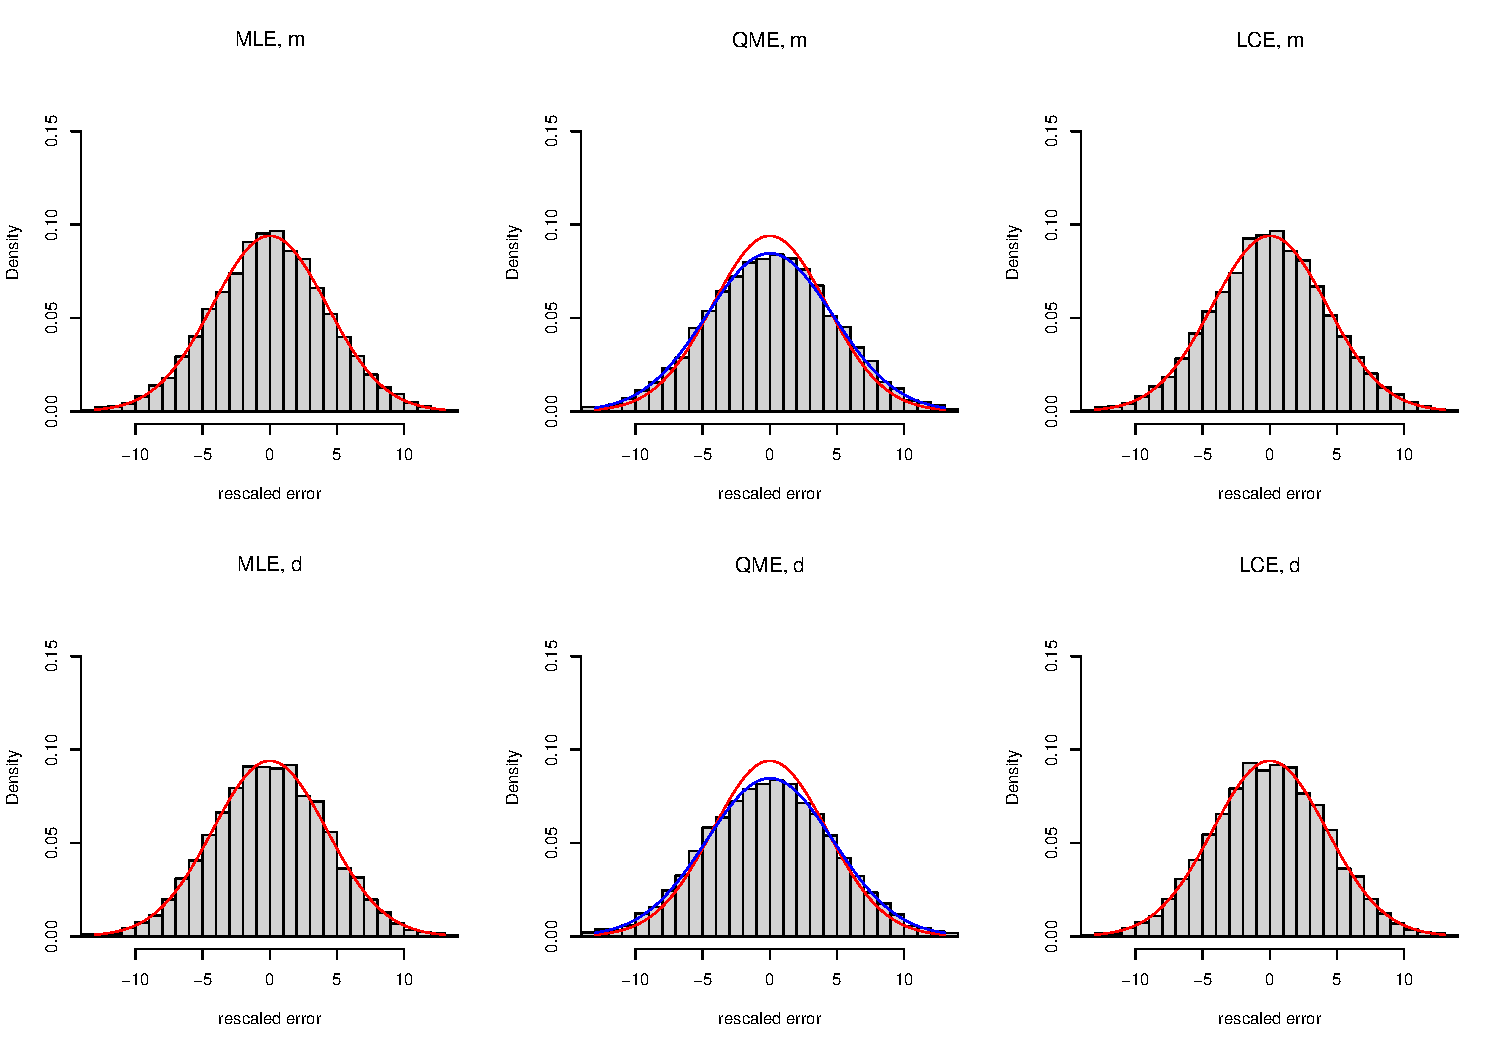
\includegraphics[width=\textwidth]{fig-Cauchy.pdf}
\caption{Histograms for the $M=10000$ Monte Carlo simulations of the rescaled statistical error of the MLE, QME, and LCE for the Cauchy distribution with $(m,d)=(2,3)$ and $n=10000$. Superimposed red and blue lines are the theoretical centered Gaussian asymptotic distributions of the MLE and the QME, respectively.}\label{fig:cauchy}
\end{figure}

It is computed faster than the sequence of MLE, as shown in Table \ref{tab:cauchy:time:cvm}.

\input{tab-Cauchy.tex}



\paragraph{P\'olya (negative binomial)}

The fourth example is the joint estimation of the size parameter $r$ and the mean parameter $\mu$ in the statistical experiment generated by a sample $(X_1,X_2,\ldots,X_n)$ of i.i.d. negative binomial random variables whose (discrete) probability density function is given by
$$ f(x)= \frac{\Gamma(r+x)}{\Gamma(r)x!} \left( \frac{r}{\mu+r} \right)^{r} \left(\frac{\mu}{\mu+r} \right)^{x}, \quad x \in \mathbb{N}.$$
Let us denote $\vartheta=(r,\mu)$. In this statistical experiment, the sequence of maximum likelihood estimators $(\widehat{\vartheta}_n, n \geq 1)$ of $\vartheta$ is not in a closed-form and the Fisher information matrix neither.

For this distribution, 
$$ m_1(\vartheta)= \mu \quad  \mbox{and} \quad  m_2(\vartheta) = \mu^2 +\mu + \frac{\mu^2}{r}$$
that gives closed-form sequence of moment estimators $(\vartheta^*_n=(r^*_n,\mu^*_n), n \geq1)$ given by
$$ r_n^*= \frac{\tilde{m}_1^2}{(\tilde{m}_2-\tilde{m}_1^2)-\tilde{m}_1} \quad  \mbox{and}  \quad \mu_n^*=\tilde{m}_1.$$


In this discrete case, the sequence of Le~Cam's one-step estimators \eqref{LC2} defined with the Hessian still overperforms the initial sequence of ME in terms of asymptotic variance (see Figure~\ref{fig:polya} and the next Table for CvM statistics). Let us mention that the CvM statistics are computed with the estimated variances for MLE and LCE.

\begin{figure}[ht]
\centering
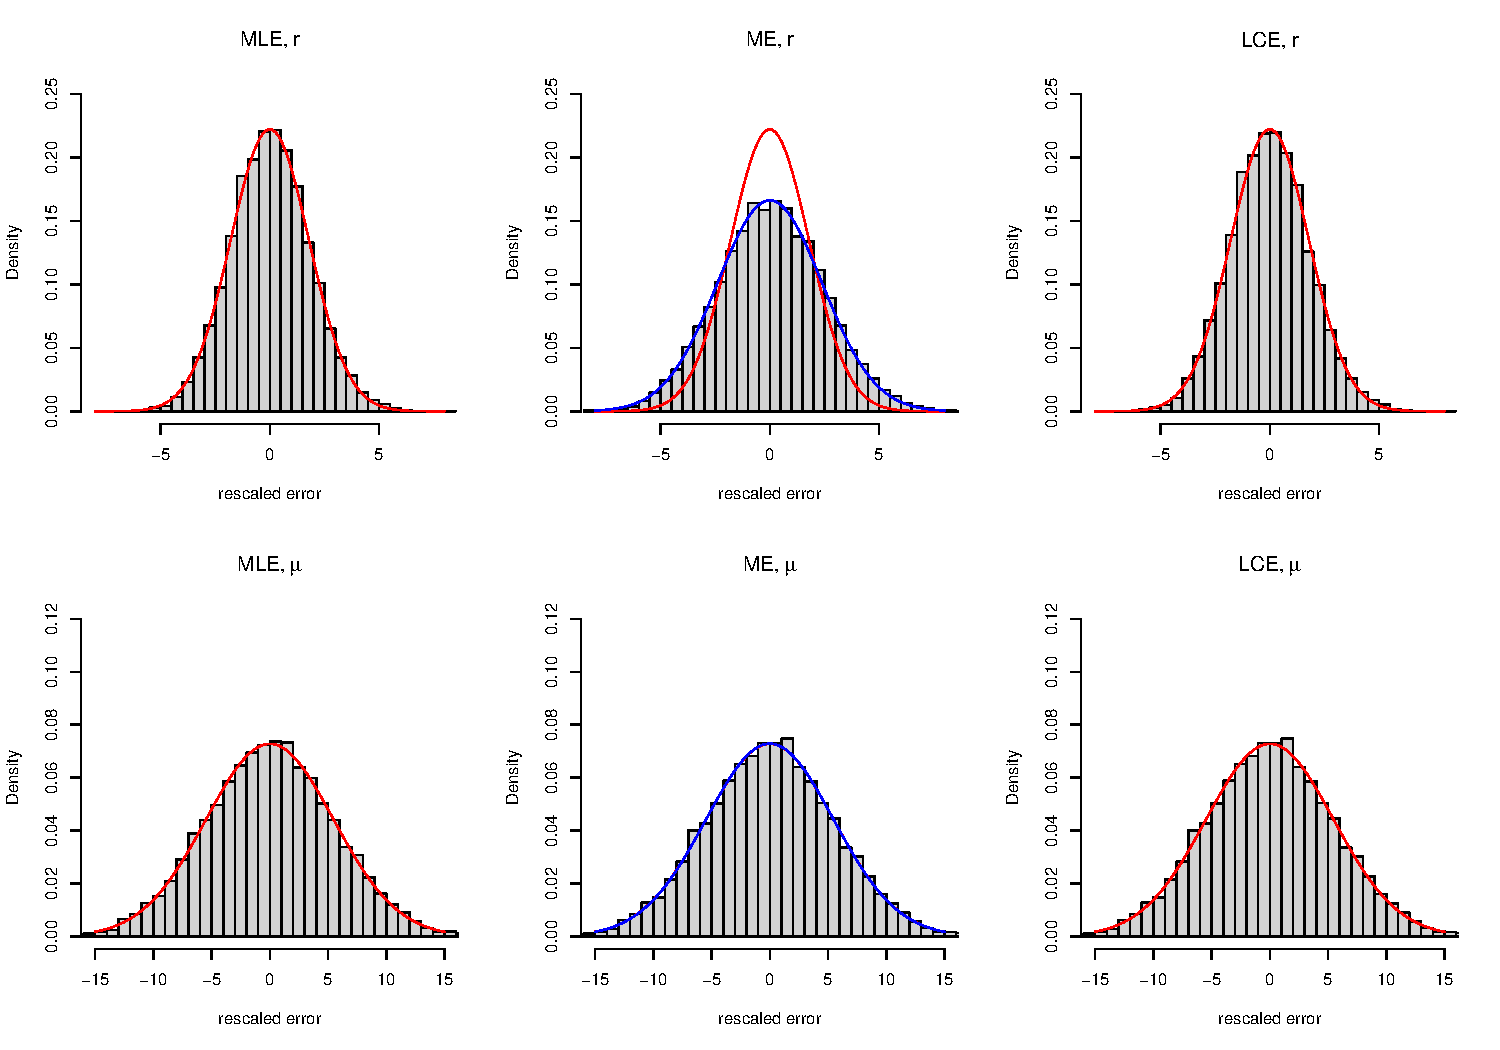
\includegraphics[width=\textwidth]{fig-nbinom.pdf}
\caption{Histograms for the $M=10000$ Monte Carlo simulations of the rescaled statistical error of the MLE, ME, and LCE for the Polya distribution with $(r,\mu)=(1,5)$ and $n=10000$. Superimposed red line is the empirical Gaussian asymptotic distributions of the MLE. Superimposed blue line is the theoretical centered Gaussian asymptotic distributions of the ME.}\label{fig:polya}
\end{figure}

It also overperforms the sequence of MLE in terms of computation time, as shown in Table \ref{tab:nbinom:time:cvm}. 

% latex table generated in R 4.0.3 by xtable 1.8-4 package
% Wed Jan  6 17:48:13 2021
\begin{table}[ht]
\centering
\begin{tabular}{rrrr}
  \hline
 & MLE & ME & LCE \\ 
  \hline
Computation time (s) & 2038.33 & 39.59 & 104.75 \\ 
  CvM statistic r & 0.18 & 0.71 & 0.19 \\ 
  CvM statistic mu & 0.05 & 0.05 & 0.05 \\ 
   \hline
\end{tabular}
\caption{Computation time and CvM statistics} 
\label{tab:nbinom:time:cvm}
\end{table}



\paragraph{Weibull}

The fifth example is the joint estimation of the shape parameter $\tau>0$ and the rate parameter $\beta>0$ in the statistical experiment generated by a sample $(X_1,X_2,\ldots,X_n)$ of i.i.d. Weibull random variables whose probability density function is given by
$$ f(x)= \beta \tau (\beta x)^{\tau-1} \exp \left( - (\beta x)^\tau \right), \quad x \in \mathbb{R}^+_*.$$
Let us denote $\vartheta=(\tau,\beta)$. In this example, neither the ME nor the MLE is in closed-form. However, the score and the Fisher information matrix can be explicitly computed. For instance,
$${\cal I}(\vartheta) = \begin{pmatrix}  \frac{1}{\tau^2} \left( \psi^{(2)}(1)+ [\psi^{(1)}(2)]^2 \right) & \frac{1}{\beta} \psi^{(1)}(2) \\  \frac{1}{\beta} \psi^{(1)}(2)
& \frac{\tau^2}{\beta^2}\end{pmatrix}.$$

Moreover, it is possible to define a closed-form initial sequence of graphical plot estimators (based on the explicit form of the cumulative distribution function). Let us denote $x_i=\log(-\log(1-i/(n+1)))$ and $Z_i=\log\left(X_{(i)}\right)$ for $i=1,\ldots,n$. The sequence of ordinary least square (OLS) based estimators $(\vartheta^*_n=(\tau^*_n, \beta^*_n), n \geq1)$ is defined by 
$$
\tau^*_n = \left(\frac{\sum\limits_{i=1}^n (x_i -\overline{x}_n)Z_i}{\sum\limits_{i=1}^n (x_i -\overline{x}_n)^2} \right)^{-1} \quad  \mbox{and} \quad \beta^*_n= \exp \left( \overline{Z}_n-(\tau^*_n)^{-1} \overline{x}_n \right),
$$
where $\overline{Z}_n$ stands for the average of $Z_1,\dots,Z_n$.


%Note that even if the ME is not explicit, direct computation of its explicit asymptotic variance can be conducted and is illustrated on the corresponding Figure~\ref{fig:weibull}.

The sequence of Le~Cam's one-step estimators overperforms the initial sequence of OLS-based estimators in terms of asymptotic variance (see Figure~\ref{fig:weibull} and the next Table). Since OLS presents a small bias for samples of finite size, its CvM statistics are bigger in the next Table. 

\begin{figure}[ht]
\centering
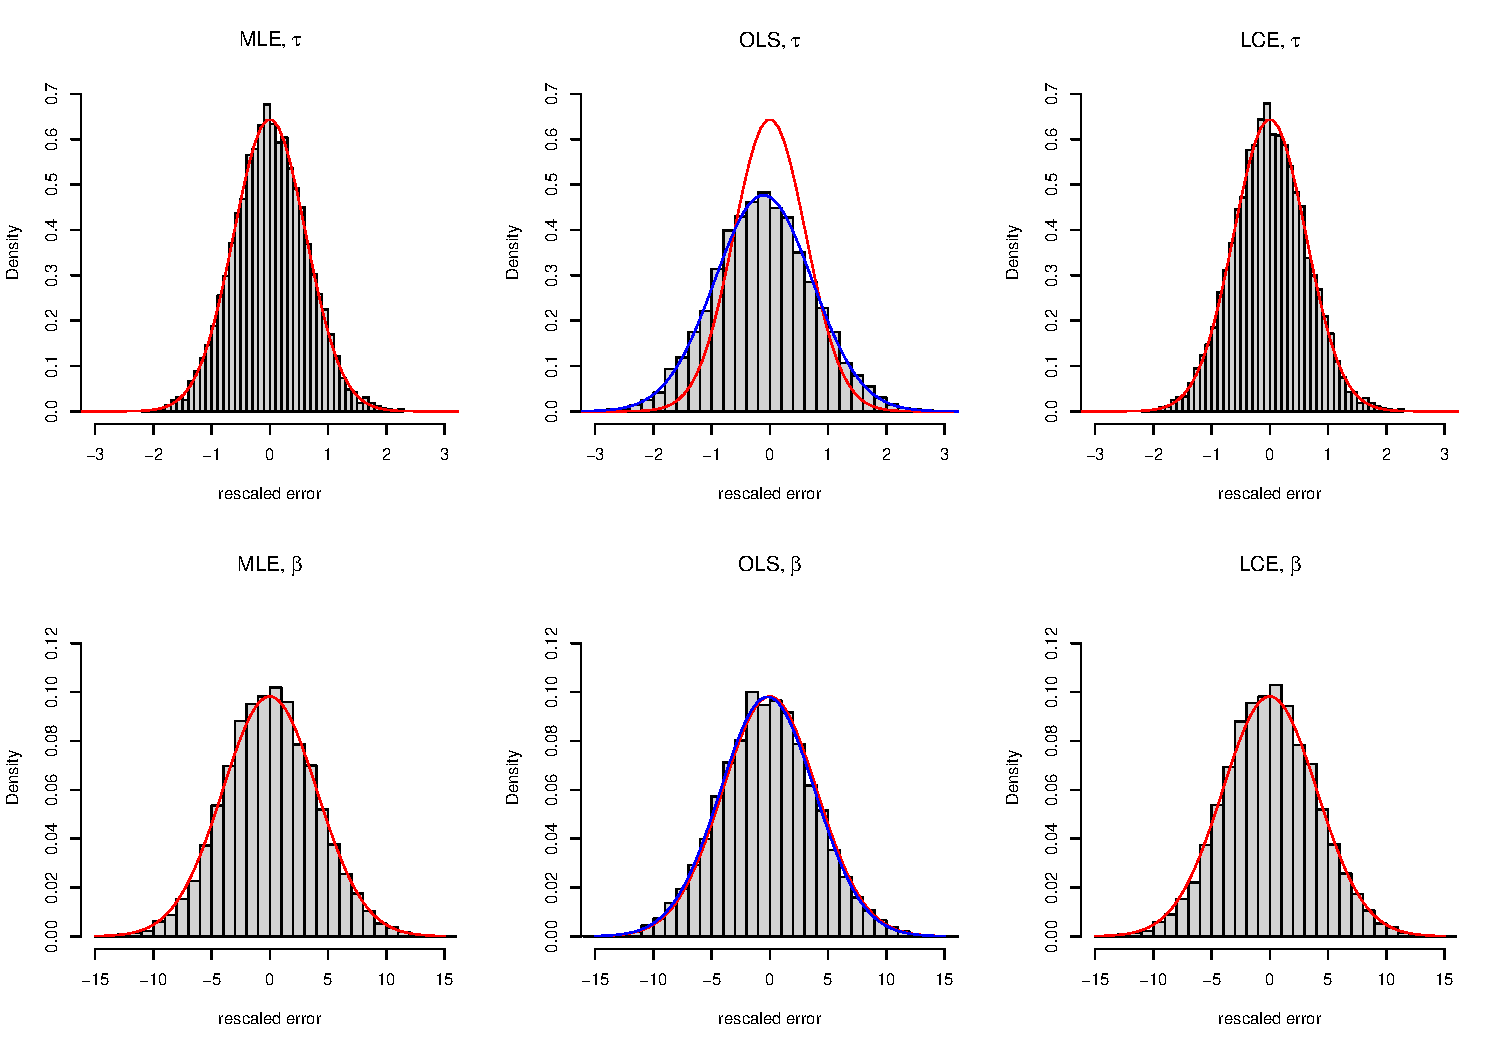
\includegraphics[width=\textwidth]{fig-Weibull.pdf}
\caption{Histograms for the $M=10000$ Monte Carlo simulations of the rescaled statistical error of the MLE, OLS, and LCE for the Weibull distribution with $(\tau,\beta)=(0.8,3)$ and $n=10000$. Superimposed red line is the theoretical centered Gaussian asymptotic distributions of the MLE. Superimposed blue line is the empirical Gaussian asymptotic distributions of the OLS.}\label{fig:weibull}
\end{figure}

It also overperforms the sequence of MLE in terms of computation time for large datasets, as shown in Table \ref{tab:weibull:time:cvm}. 

\input{tab-Weibull.tex}


\subsection{Numerically computed initial sequence of guess estimators and numerical computations in the generic case}\label{sec:improved}

As soon as the ME is not in closed form or no other closed form estimators can be elicited, the use of a numerical ME as an initial sequence of guess estimator in Le~Cam's one-step procedure is difficult to justify. Indeed, no gain will be given in terms of time computation and the use of the MLE is finally equivalent. We propose  therefore to use in the \pkg{onestep} function  an improvement of the classical Le Cam procedure.

Indeed, it can be shown (see \cite{KU15} or \cite{KutMotrun}) that for a $n^{\delta/2}$--consistent initial sequence of guess estimators (with $\frac12 < \delta \leq 1$) and a Lipshitz Fisher information matrix, the sequence of Le Cam's one-step estimators
is also consistent, asymptotically normal and efficient (in the Fisher sense). In this setting, for a initial sequence which is neither asymptotically rate nor variance efficient, the new sequence is asymptotically rate and variance  efficient.

This result allows one to use the numerical computation of the MLE on a subsample (of size $n^\delta$, for $\frac12 < \delta \leq 1$) as an initial sequence of guess estimators. Namely, for this initial sequence of guess estimators $(\vartheta^*_n, n\geq 1)$, 
$$ n^{\frac{\delta}{2}} \left( \vartheta^*_n-\vartheta \right) \rightarrow {\cal N}\left(0,{\cal I}(\vartheta)^{-1}\right).$$

Then the sequence of Le~Cam's one-step estimators given by \eqref{LC2} is also consistent, asymptotically normal and efficient (in the Fisher sense) with
$$ \sqrt{n}\left( \widehat{\vartheta}_n-\vartheta \right) \rightarrow {\cal N}\left(0,{\cal I}(\vartheta)^{-1}\right).$$

The choice of the exponent $\delta$ that measures the size of the subsample $ \frac12 <\delta \leq 1$ is set to 0.9 by default and can be chosen by the user with the parameter \code{control}, for instance in the call

$$\texttt{onestep(data, distr, control=list(delta=0.7))}$$


The example of Pareto II distribution is interesting and shows the gain in terms of variance (with respect to the initial sequence of guess estimators) and in terms of computation time in comparison with the MLE. 

This improved method is also used when the distribution does not belong to the closed-formula family. 
The initial sequence of maximum likelihood estimators is computed on a subsample with the \code{mledist} function of the \pkg{fitdistrplus} package. The score and the Hessian in the Newton step of the Le Cam procedure \eqref{LC2} are numerically 
computed with the functions \code{grad} and \code{hessian} of the \pkg{numDeriv} 
package (see \cite{numDeriv19}).


\paragraph{Pareto II}

The sixth example is the joint estimation of the shape parameter $\alpha>0$ and the scale parameter $\sigma>0$ in the statistical experiment generated by a sample $(X_1,X_2,\ldots,X_n)$ of i.i.d. Pareto II (Lomax) random variables whose probability density function is given by
$$ f(x)= \frac{\alpha \sigma^\alpha}{(\sigma + x)^{\alpha+1}}, \quad x \in \mathbb{R}^+.$$


In this example neither the ME (when it exists for $\alpha>2$) nor the MLE are in closed-form. But the score and the Fisher information matrix can be explicitly computed. 

Let $\vartheta=(\alpha,\sigma)$. Then, considering the MLE computed on a subsample of size $n^\delta$, $\frac12 < \delta \leq 1$, as an initial sequence of guess estimators $(\vartheta_n^*, n \geq 1)$,  we get
$$ n^{\frac{\delta}{2}} \left( \vartheta^*_n-\vartheta \right) \rightarrow {\cal N}\left(0,{\cal I}(\vartheta)^{-1}\right)$$
with
$${\cal I}(\vartheta) = \begin{pmatrix} \frac{\alpha}{\sigma^2(\alpha+1)} & -\frac{1}{\sigma(\alpha+1)} \\
 -\frac{1}{\sigma(\alpha+1)} & \frac{1}{\alpha^2}\end{pmatrix}.$$
The computation of the Fisher information matrix can be found in \cite{B2003}.

Here again, the sequence of Le~Cam's one-step estimators naturally overperforms the initial sequence of MLE computed on a subsample in terms of asymptotic variance (see Figure~\ref{fig:pareto} and the next Table for the CvM statistics).

\begin{figure}[ht]
\centering
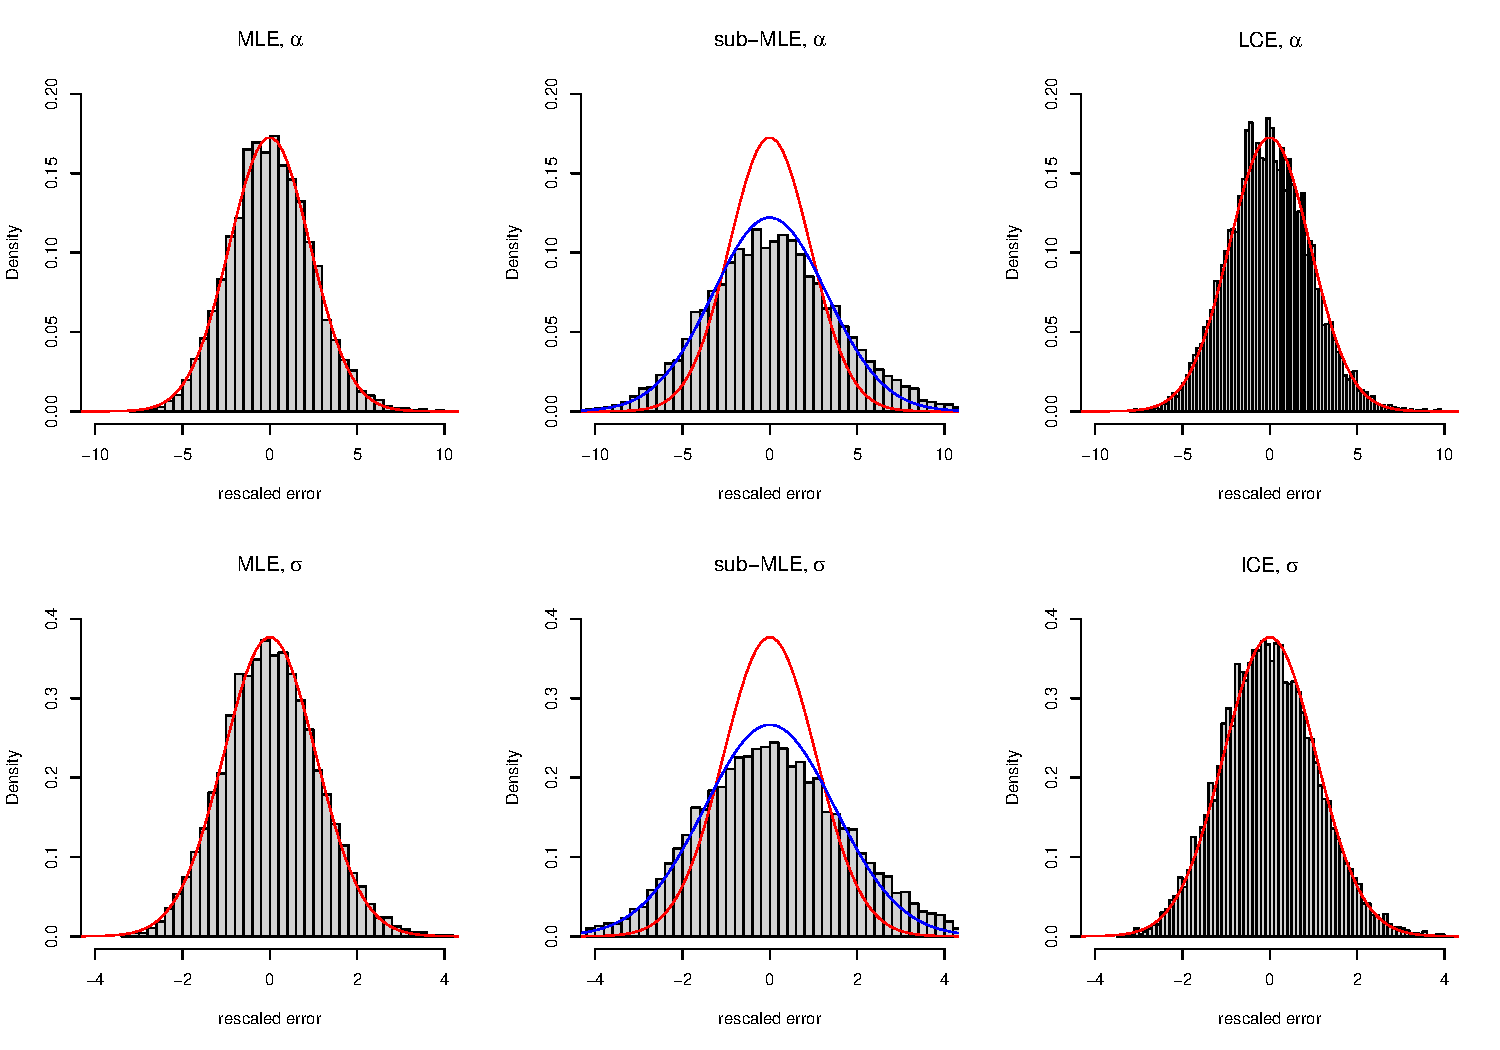
\includegraphics[width=\textwidth]{fig-Pareto.pdf}
\caption{Histograms for the $M=10000$ Monte Carlo simulations of the rescaled statistical error of the MLE, ME, and LCE for the Pareto II distribution with $(\alpha,\sigma)=(1.1,0.3)$ and $n=10000$. Superimposed red and blue lines are the theoretical centered Gaussian asymptotic distributions of the MLE and the MLE on a subsample, respectively.}\label{fig:pareto}
\end{figure}

It is also computed faster than the sequence of MLE, as shown in Table \ref{tab:pareto:time:cvm}.

\input{tab-Pareto.tex}


\paragraph{Generic function}

For the generic example, we study the Weibull distribution again and force it to be numerically computed with the function parameter \code{method="numeric"} in order not to use the closed form processing. 

We recall that, in the generic procedure, the score and the Hessian in the Newton step of the Le Cam procedure~\eqref{LC2} are numerically computed with the functions \code{grad} and \code{hessian} of the \pkg{numDeriv} package.  By default, the initial sequence of maximum likelihood estimators is computed on a subsample if size $n^\delta$ with $\delta=0.9$.


The numerically computed sequence of Le~Cam's one-step estimators reaches asymptotic efficiency for a simulation of $M=10000$ Monte-Carlo replications of samples of size $n=10000$ as shown by the CvM statistics summarized in the next table. It is still computed faster than the sequence of MLE, see Table \ref{tab:weibull:generic:time:cvm}.


\input{tab-Weibull-generic.tex}


%\begin{figure}[ht]
%\centering
%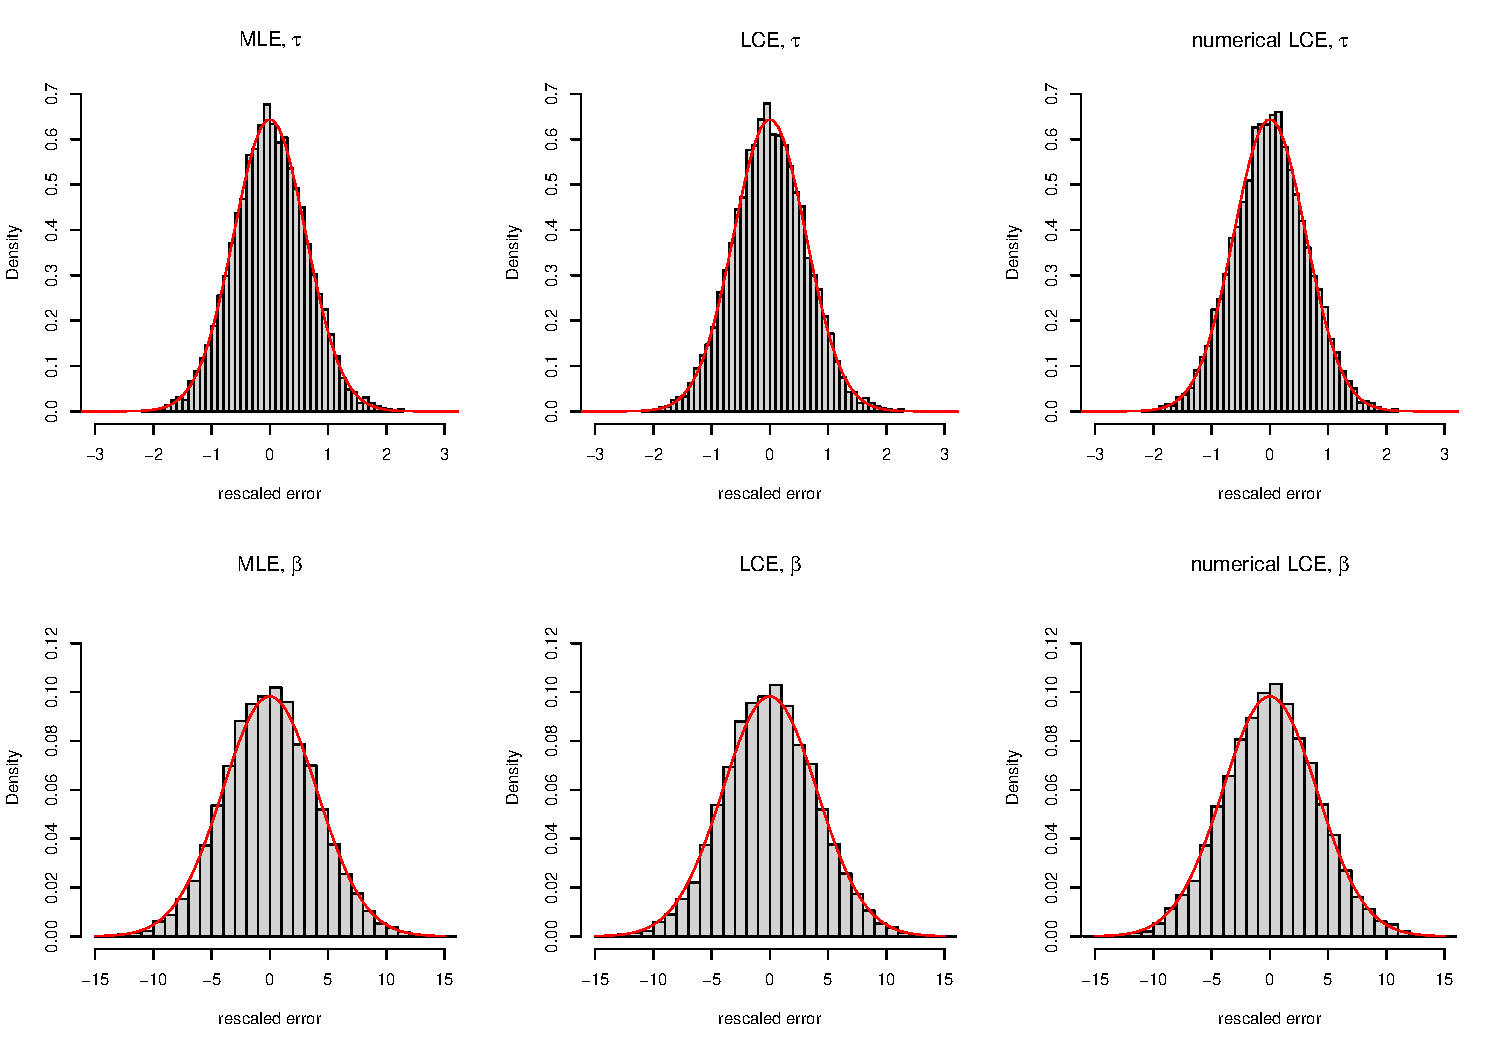
\includegraphics[width=\textwidth]{fig-Weibull-generic.pdf}
%\caption{Histograms for the MLE, ME and the generic LCE for the Weibull distribution}\label{fig:weibgeneric}
%\end{figure}

%\input{../test/Weibull-generic.out}


%\begin{example}
%N<-1000
%p<-4
%\end{example}

\noindent {\bf{Acknowledgements}} We would like to thank Yury Kutoyants and Marius Soltane for fruitful discussions on the topic. We also thank the referees for their valuable comments that improve the paper.


\bibliography{RJreferences}

\address{Alexandre Brouste\\
  Laboratoire Manceau de Math\'ematiques, Le Mans Universit\'e\\
  Avenue Olivier Messiaen, 72085 LE MANS\\
	France\\
  ORCID: 0000-0001-6719-7432\\
  \email{Alexandre.brouste@univ-lemans.fr}}
  

\address{Christophe Dutang\\
	CEREMADE, CNRS, Universit\'e Paris-Dauphine, Universit\'e PSL\\
  Place du Mar\'echal de Lattre de Tassigny, 75016 PARIS\\
	France\\
  ORCID: 0000-0001-6732-1501\\
  \email{christophe.dutang@dauphine.psl.eu}}
  
\address{Darel Noutsa Mieniedou\\
  Laboratoire Manceau de Math\'ematiques, Le Mans Universit\'e\\
  Avenue Olivier Messiaen, 72085 LE MANS\\
	France}
  
  